\documentclass[pi.tex]{subfile}


\begin{document}

\chapter*{LAMPIRAN}
\addcontentsline{toc}{chapter}{LAMPIRAN}
\setcounter{section}{0}
\renewcommand*{\theHsection}{chX.\the\value{section}}

\setcounter{page}{1}
\renewcommand{\thepage}{L-\arabic{page}}

\section{Output Program}

\begin{figure}[H]
    \centering
  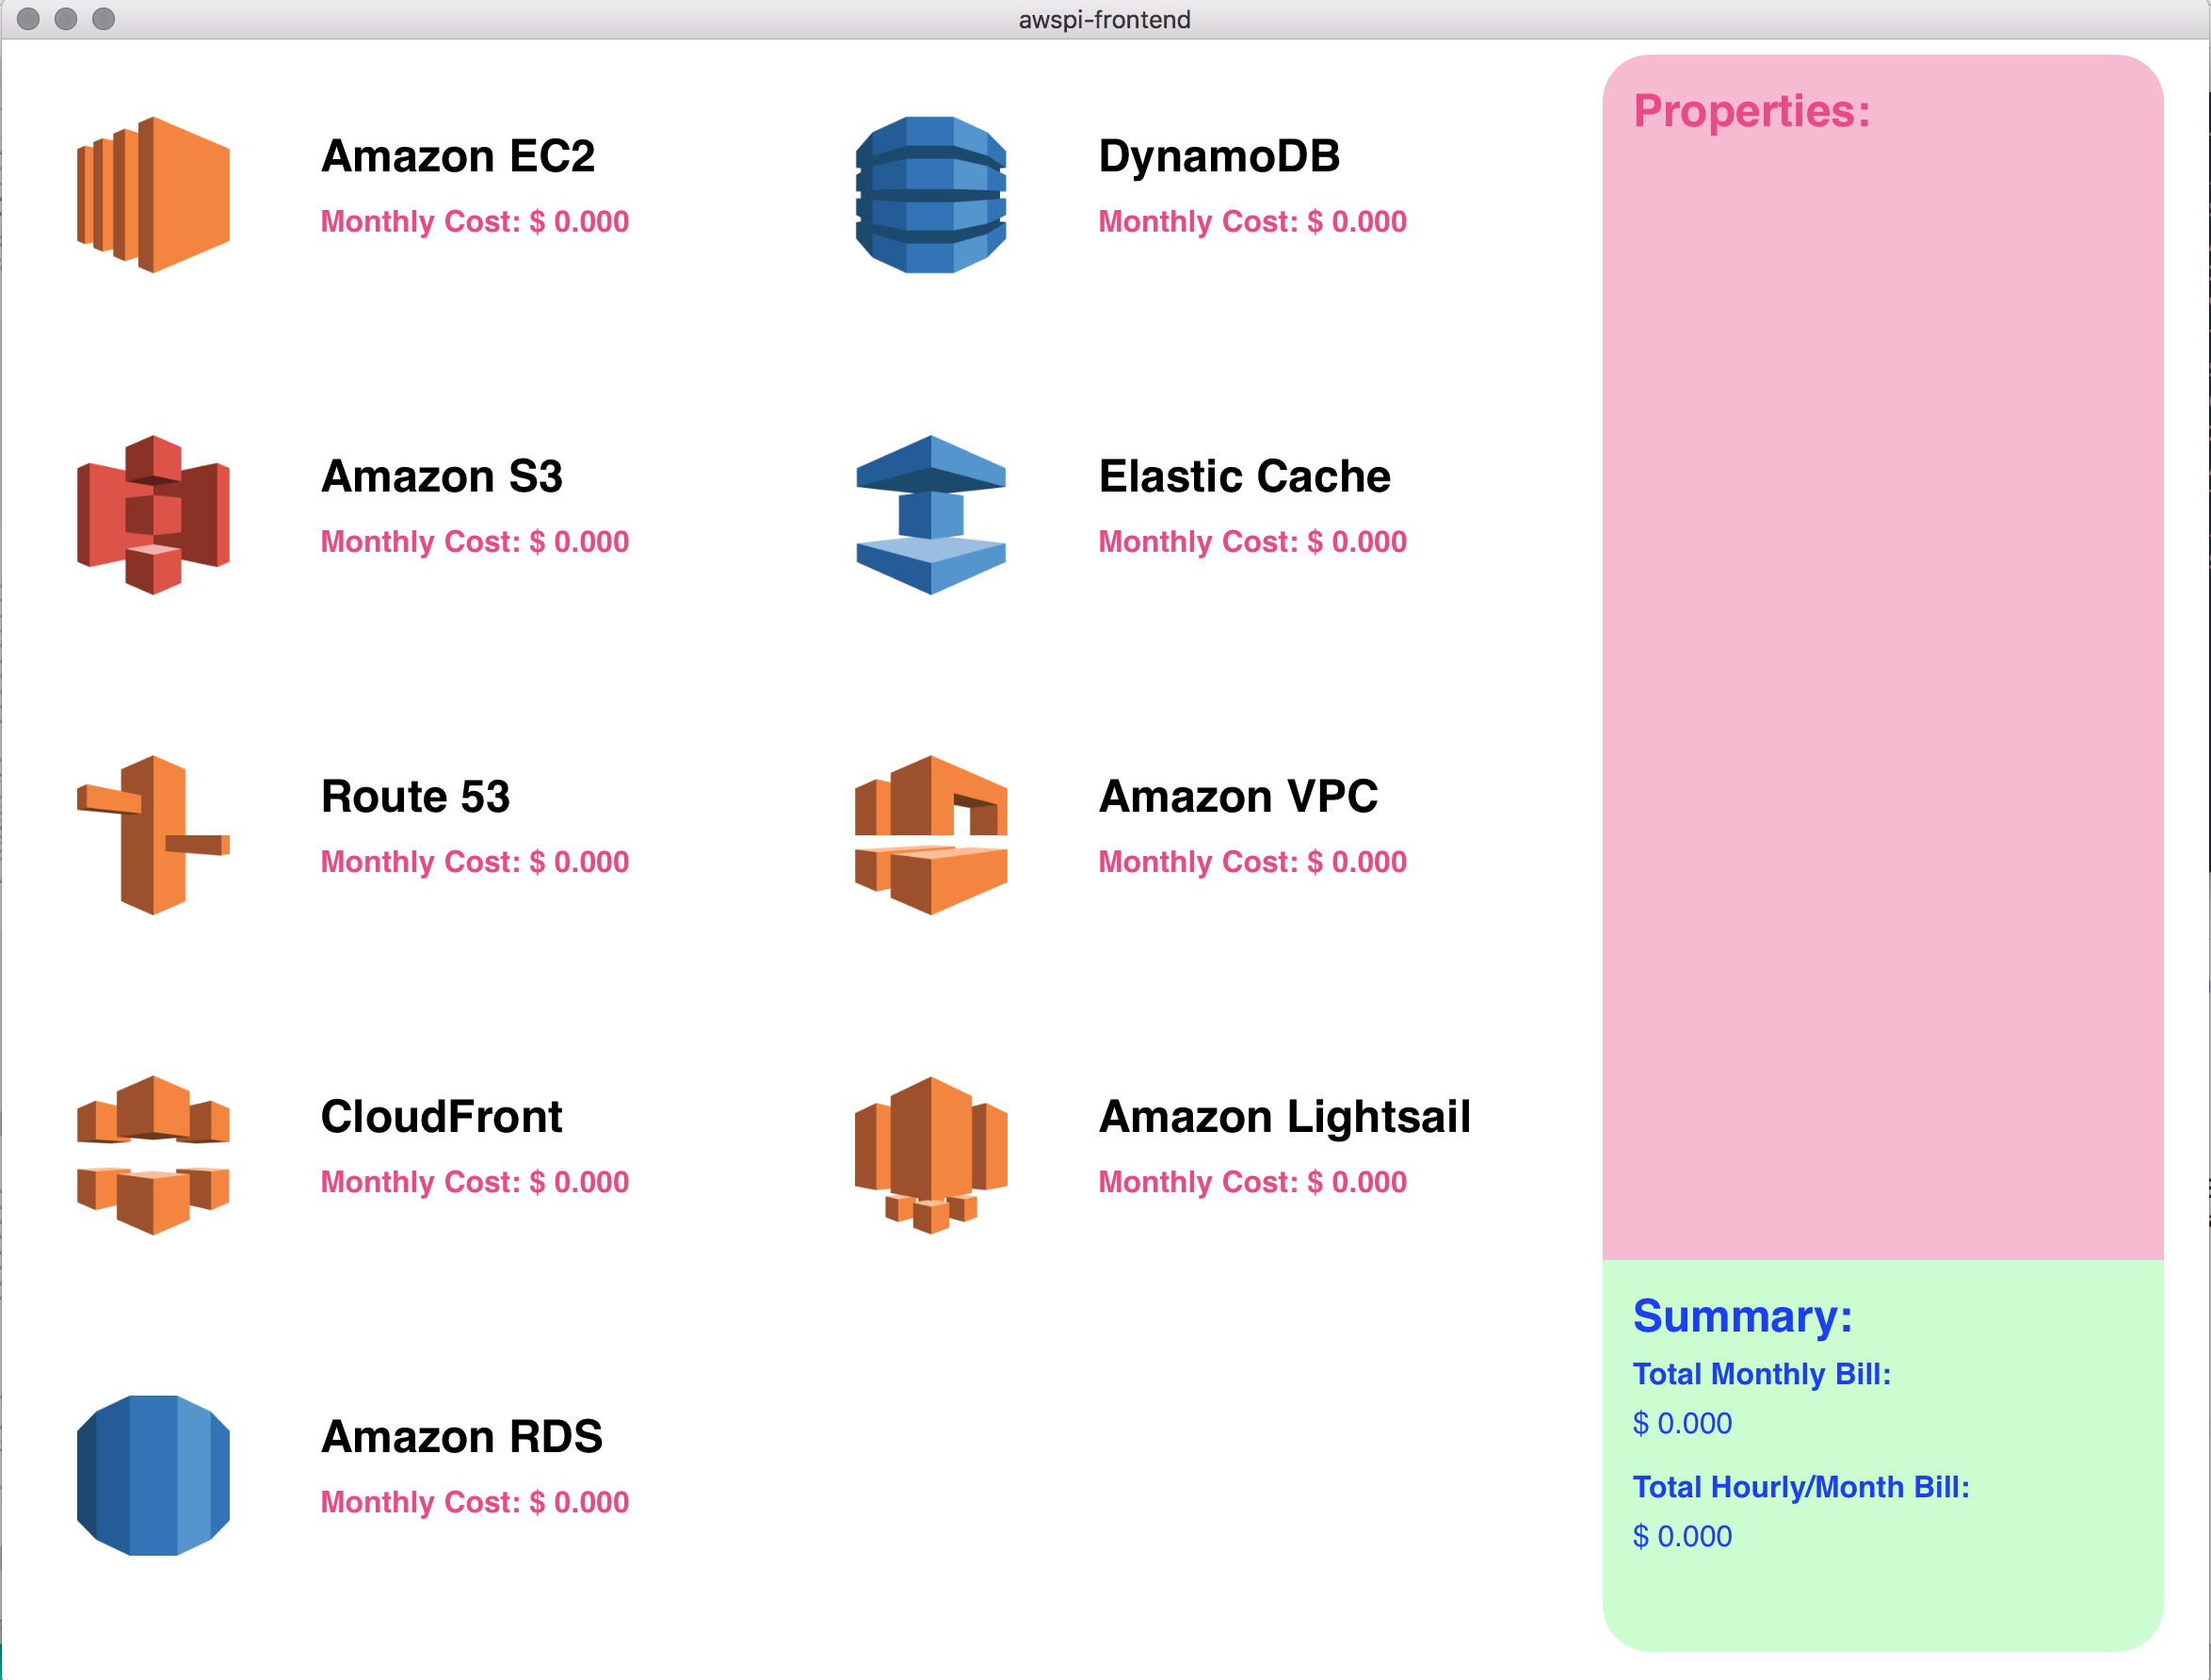
\includegraphics[width=15cm, height=10cm]{output1.png}
  \caption[Output Program Berjalan]{Tampilan Awal Aplikasi Berjalan}
\end{figure}

\begin{figure}[H]
    \centering
  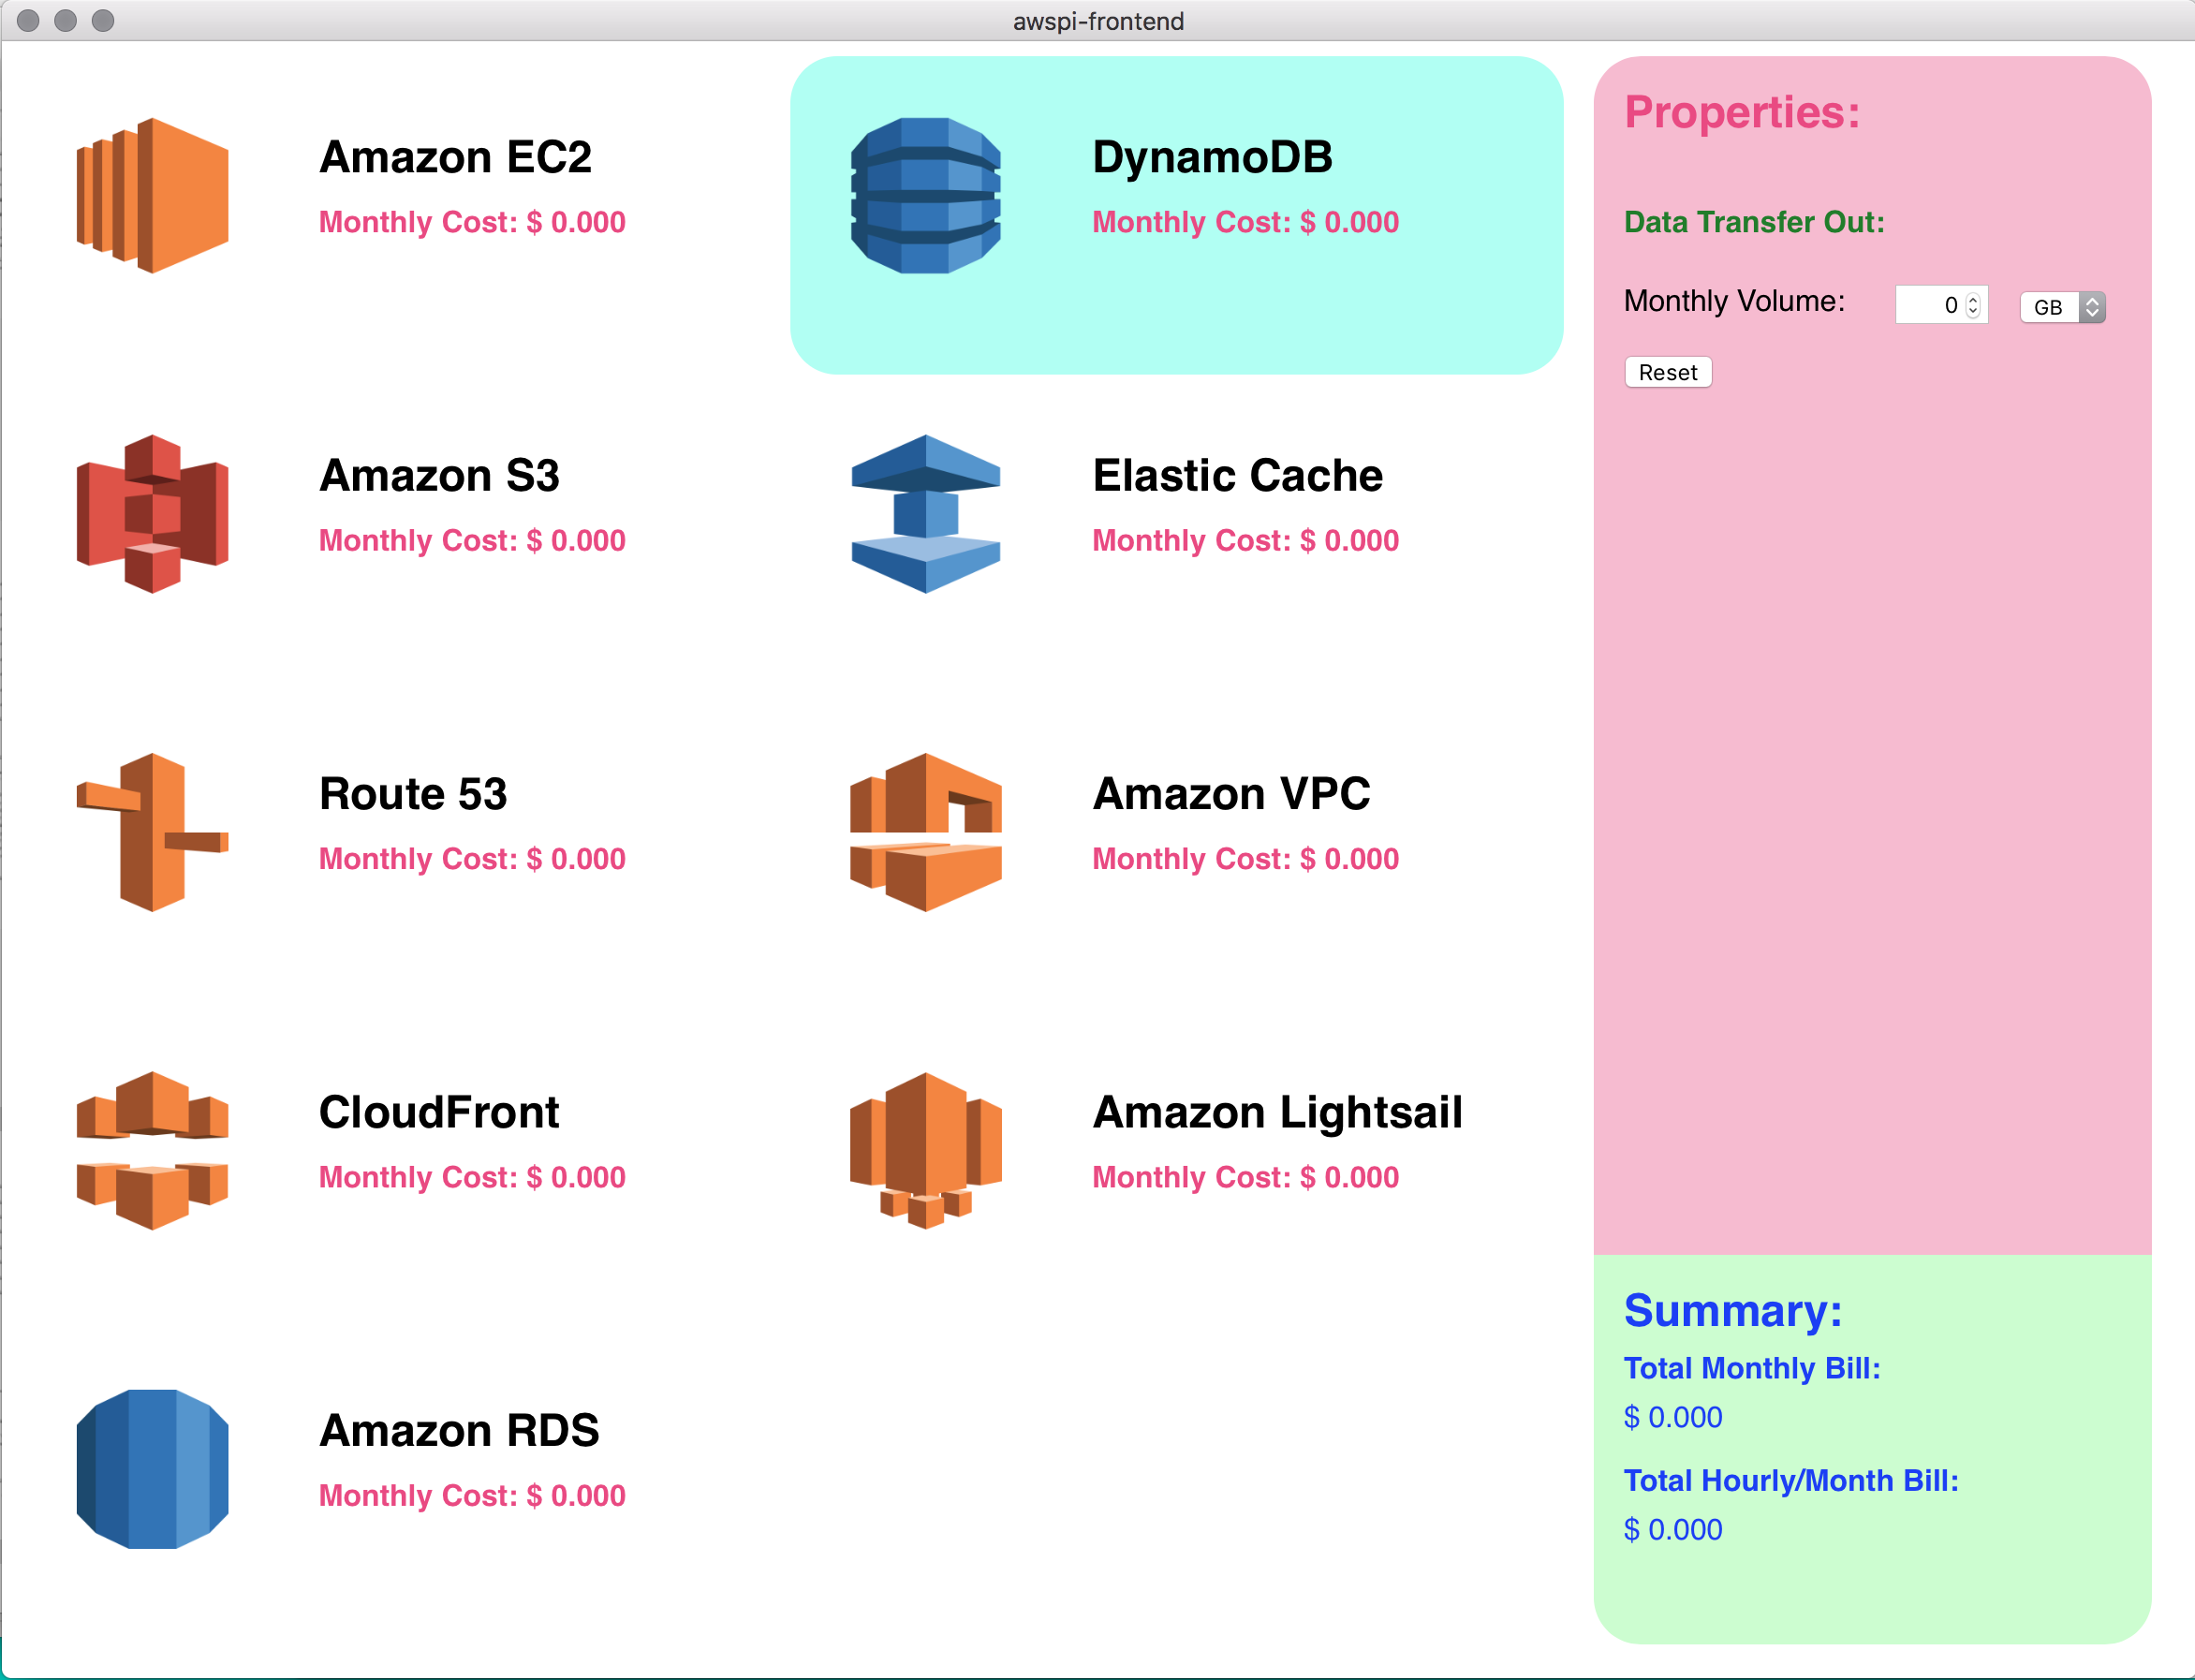
\includegraphics[width=15cm, height=10cm]{output2.png}
  \caption[Output Program Menu DynamoDB]{Tampilan Menu DynamoDB Dipilih}
\end{figure}

\begin{figure}[H]
    \centering
  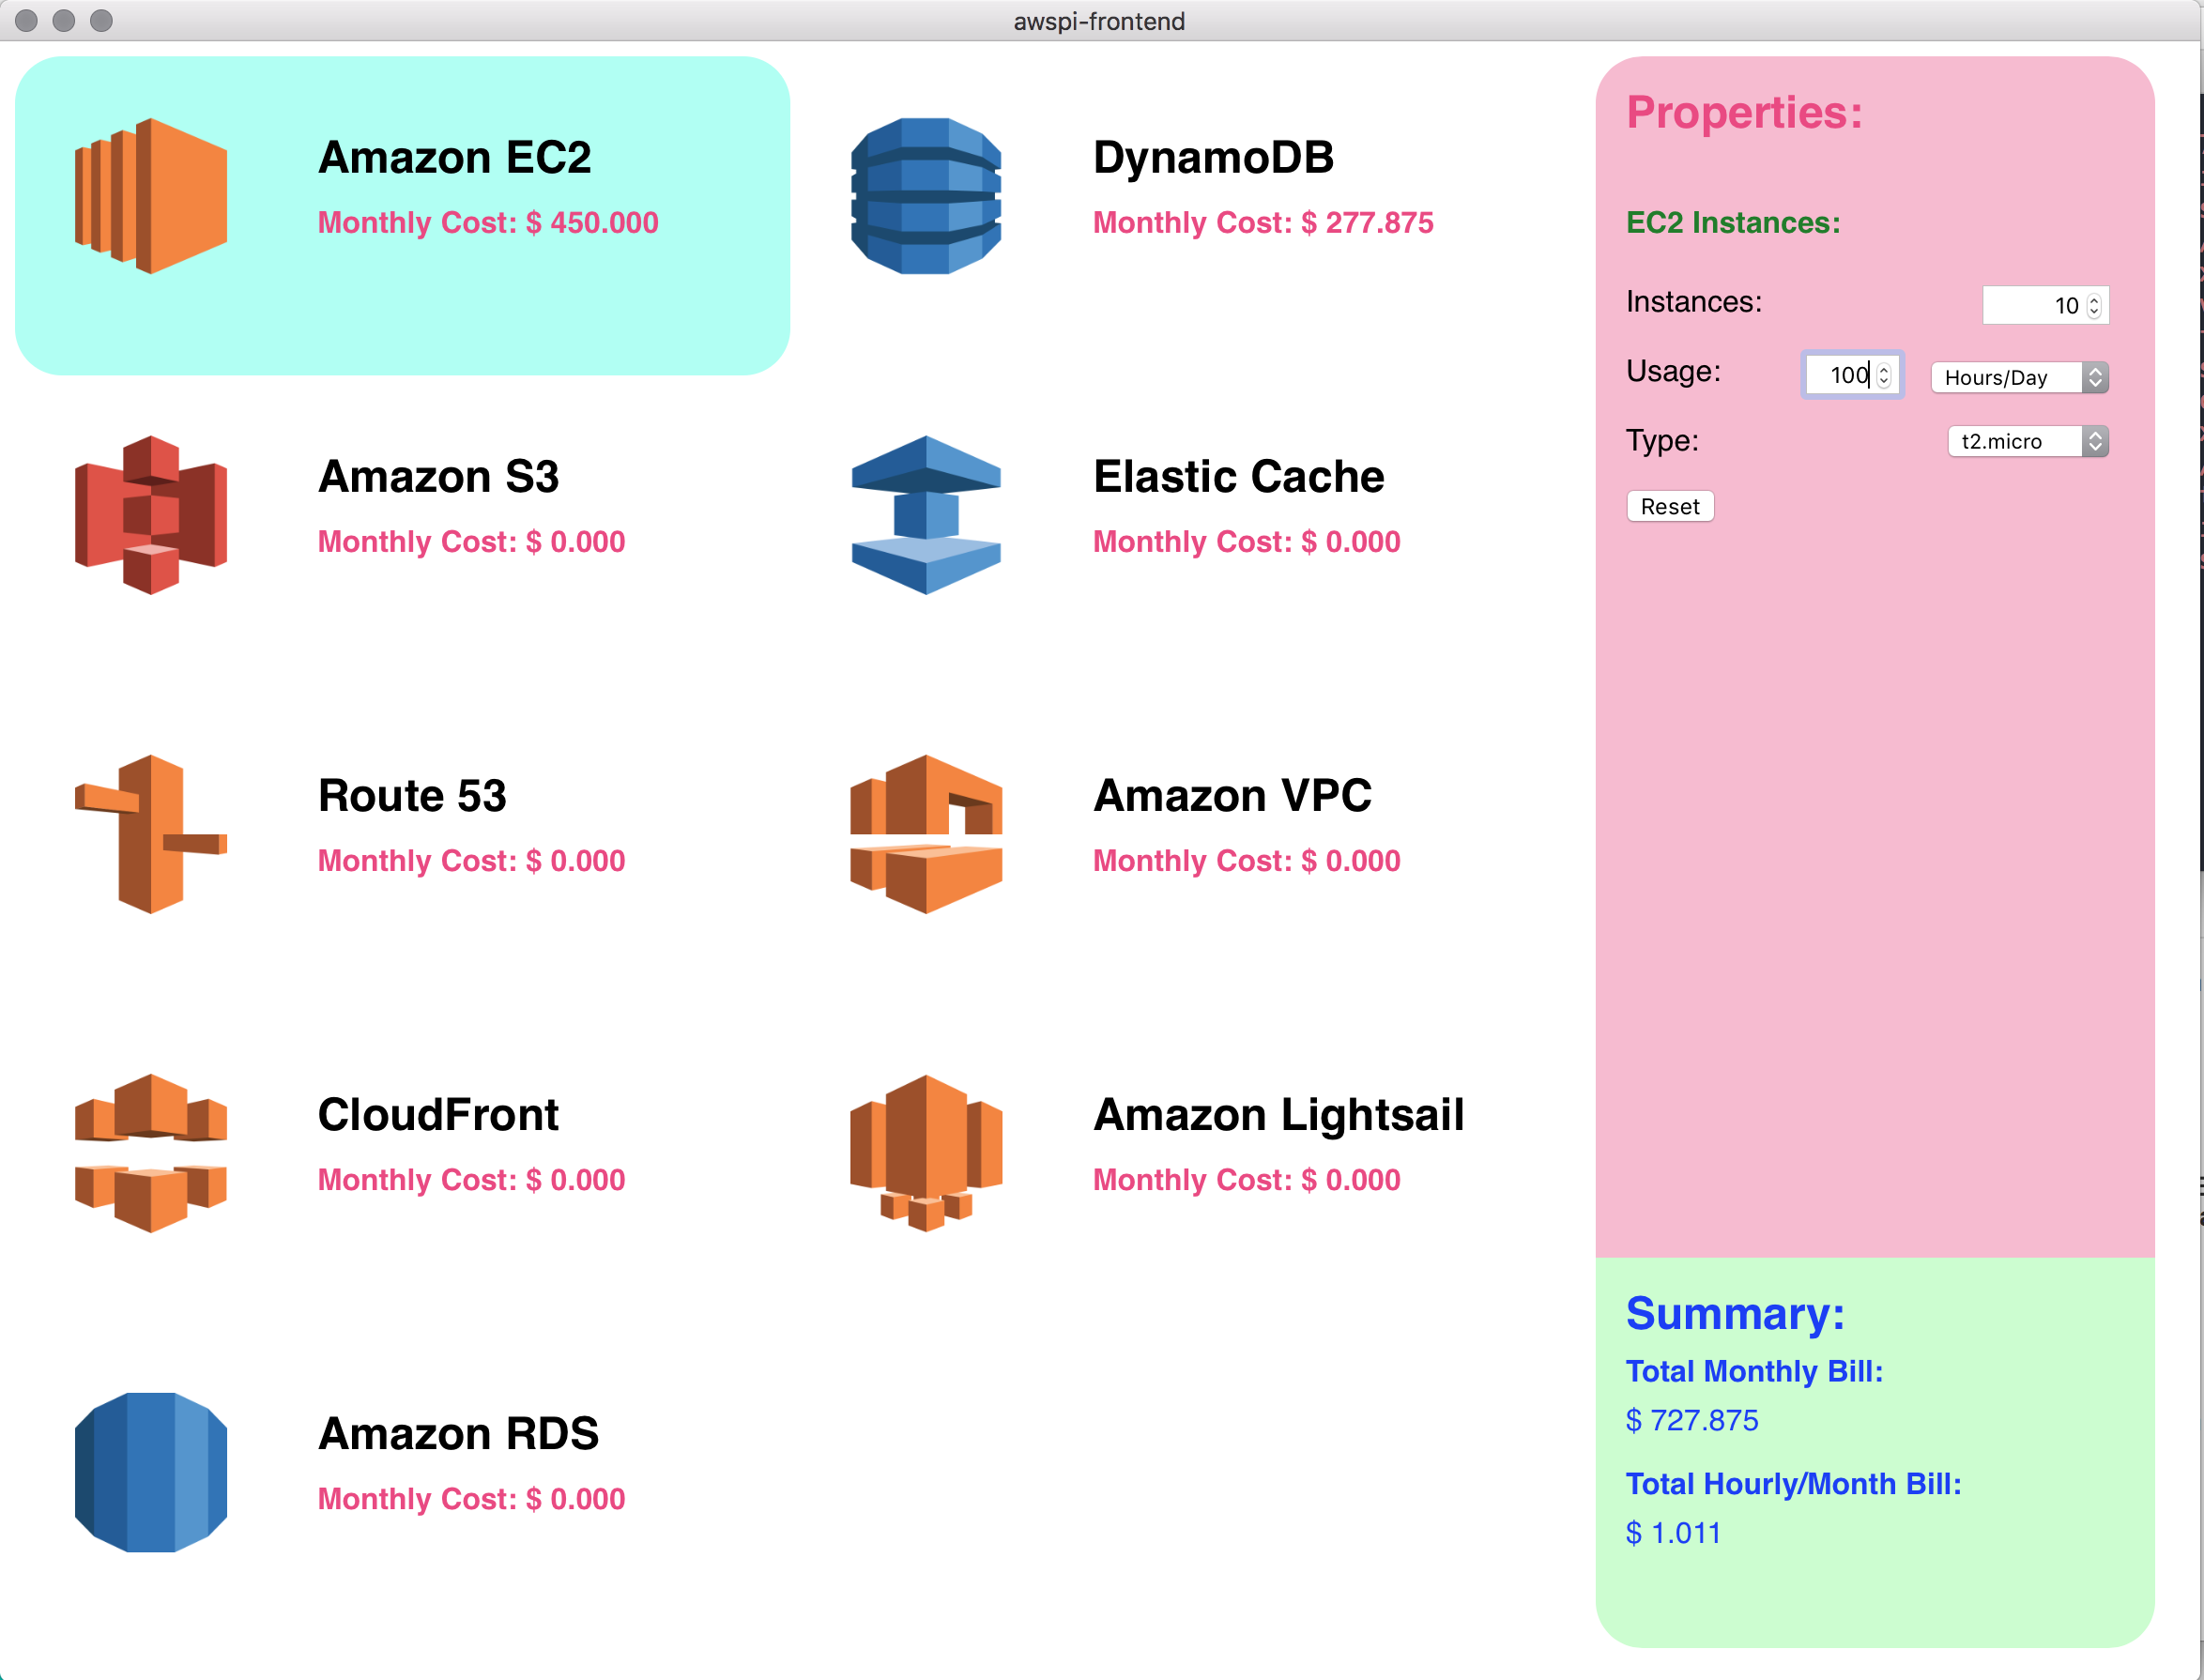
\includegraphics[width=15cm, height=10cm]{output3.png}
  \caption[Output Program Menu EC2]{Tampilan Menu EC2 Dipilih}
\end{figure}

\begin{figure}[H]
    \centering
  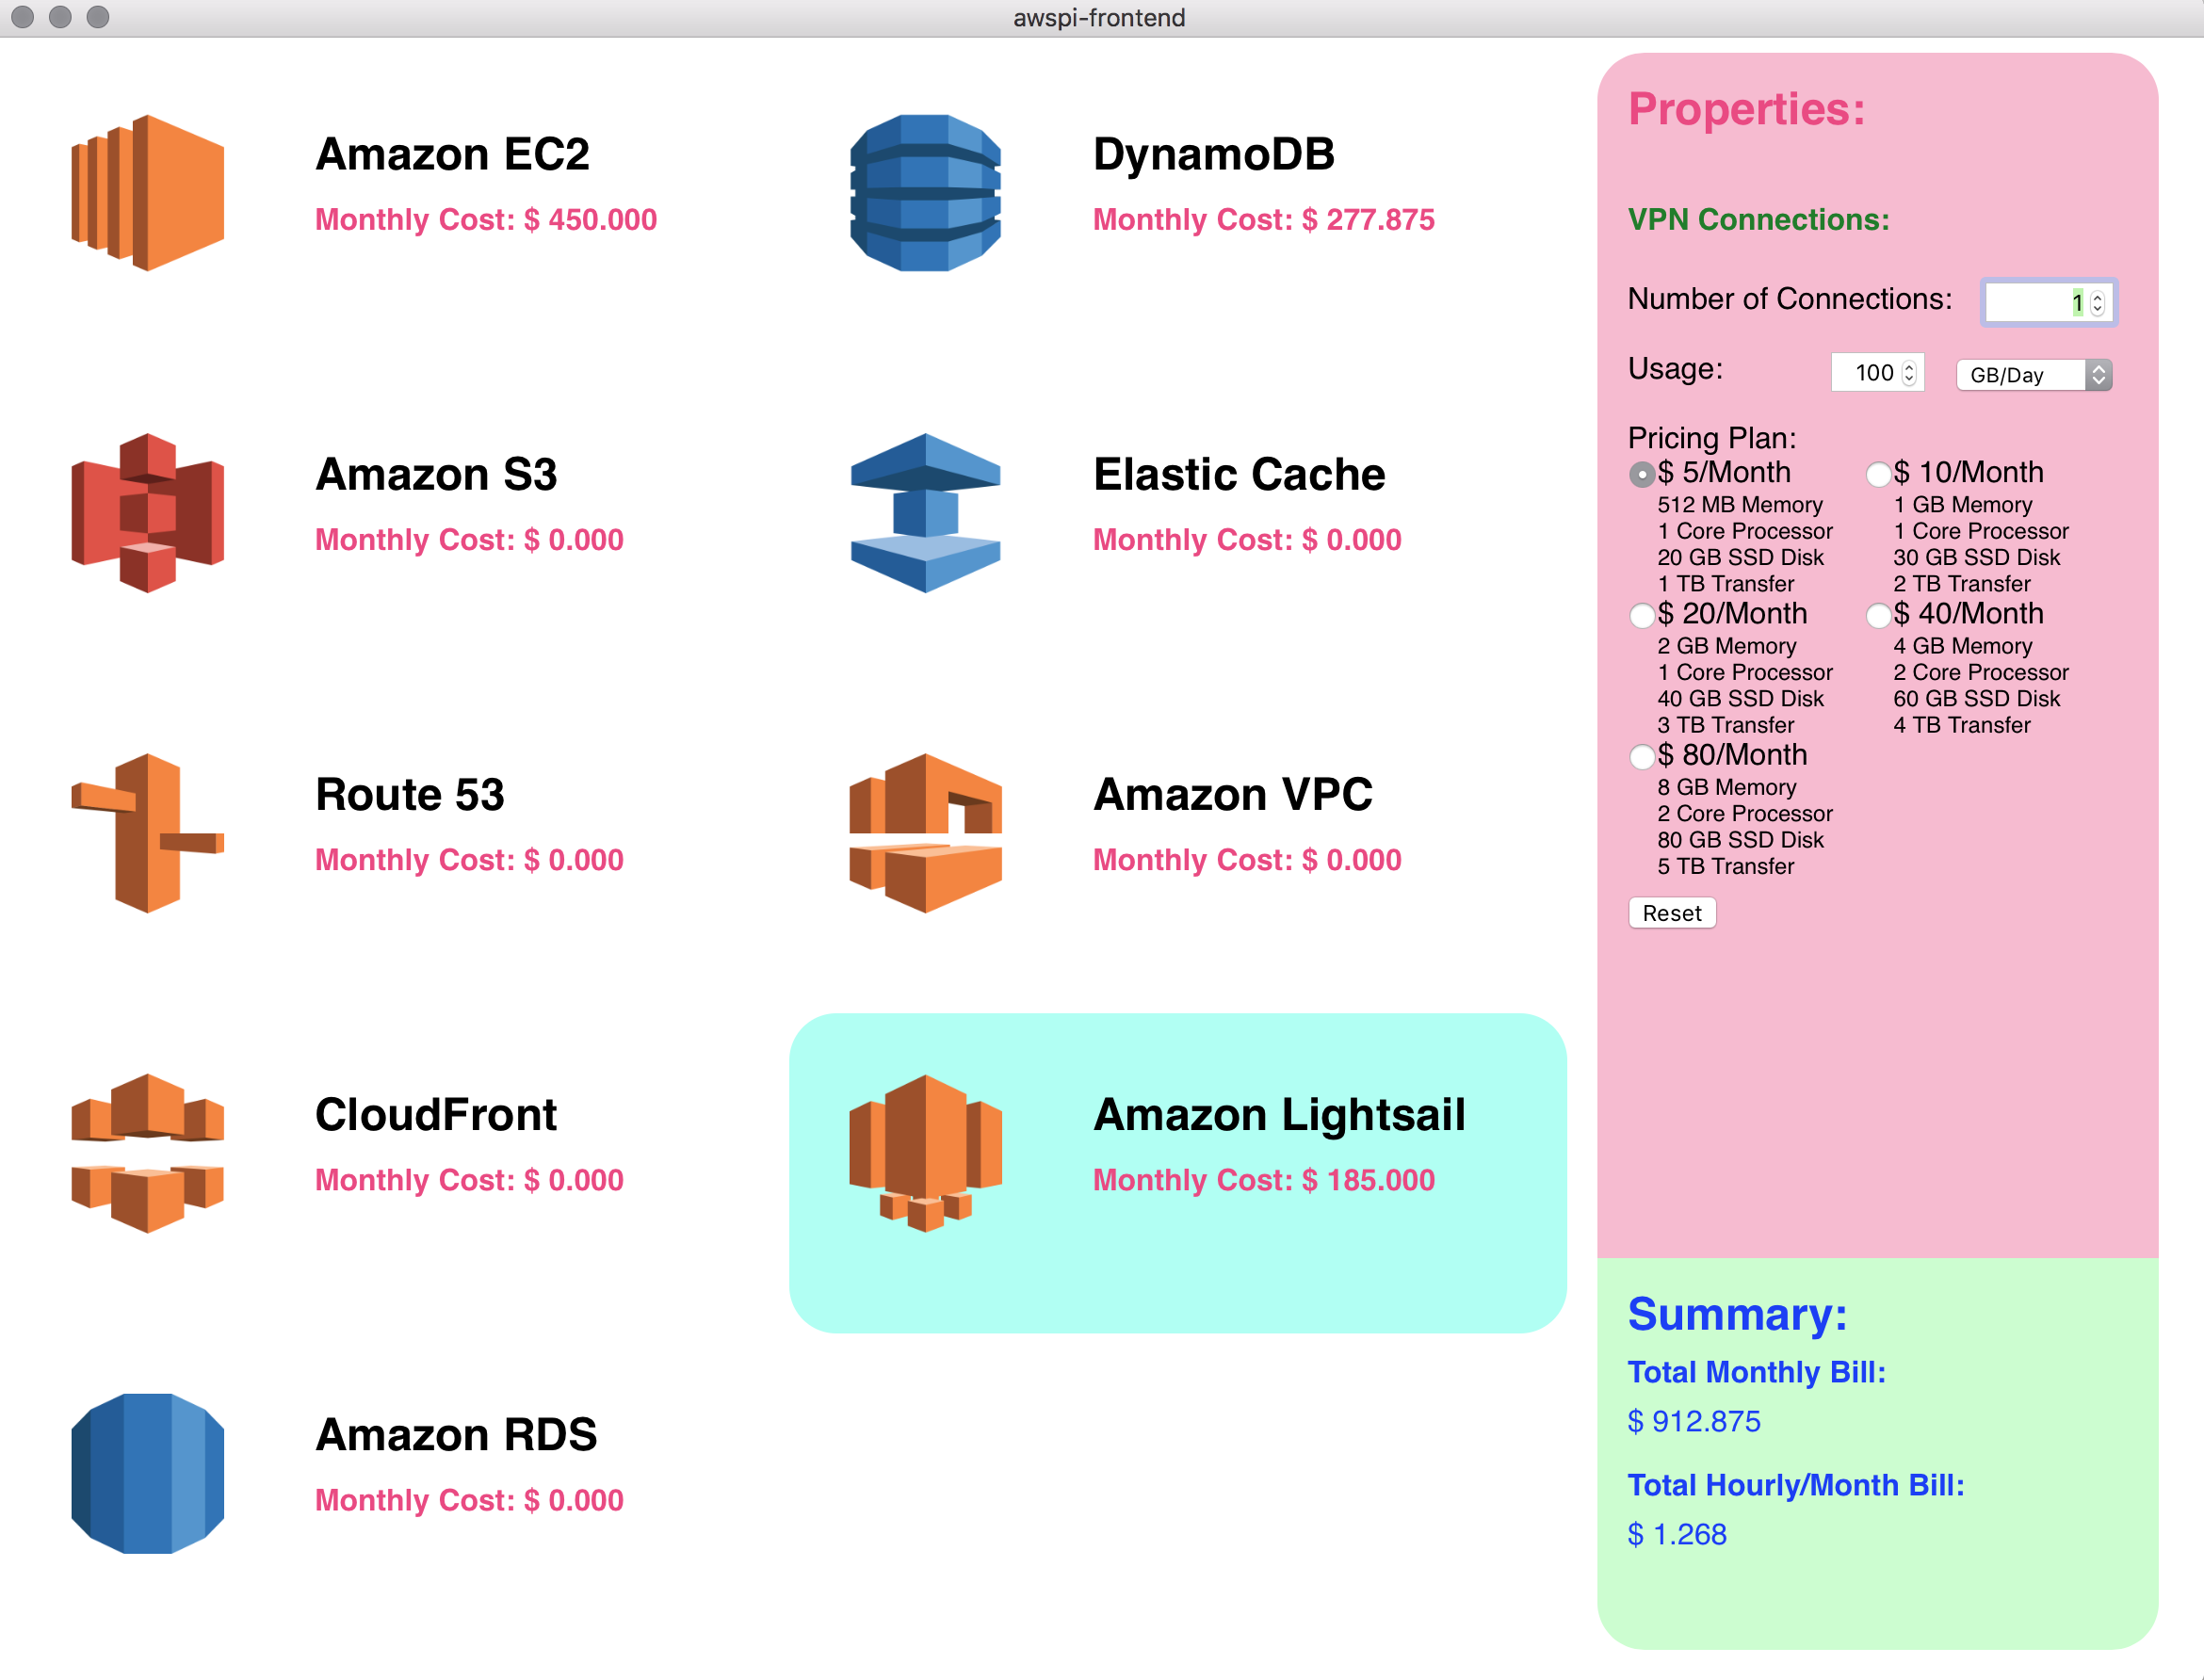
\includegraphics[width=15cm, height=10cm]{output4.png}
  \caption[Output Program Menu LightSail]{Menu LightSail Dipilih}
  \end{figure}

\pagebreak
\section{Listing Program}

Main.hs:
\begin{lstlisting}[language=Haskell]
{-# LANGUAGE OverloadedStrings, RecursiveDo, ScopedTypeVariables, FlexibleContexts, TypeFamilies, ConstraintKinds #-}

import Prelude hiding (mapM, mapM_, all, sequence)

import           Control.Monad hiding (mapM, mapM_, forM, forM_, sequence)
import qualified Data.Map                  as Map
import           Data.Monoid ((<>))
import GHCJS.DOM.Types (JSM)

import Reflex
import Reflex.Dom.Core
import Language.Javascript.JSaddle.WKWebView (runFile)
------

import AWSFunction
import Frontend.Properties.EC2
import Frontend.Properties.S3
import Frontend.Properties.R53
import Frontend.Properties.CF
import Frontend.Properties.RDS
import Frontend.Properties.DDB
import Frontend.Properties.EC
import Frontend.Properties.VPC
import Frontend.Properties.LS

------------------
-- View
------------------

main :: IO ()
main = runFile "index.html" "" mainWk

mainWk :: JSM ()
mainWk = mainWidgetWithHead headElement bodyElement

headElement :: MonadWidget t m => m ()
headElement = do
  el "title" $ text "AWS Simulator"
  styleSheet "static/stylesheet/simple.css"
 where
    styleSheet link' = elAttr "link" (Map.fromList [
        ("rel", "stylesheet")
      , ("type", "text/css")
      , ("href", link')
     ]) $ return ()

bodyElement :: MonadWidget t m => m ()
bodyElement = elClass "div" "container" $ do
  rec
-- Menu utama pemilihan jasa AWS yang paling umum digunakan
    midM <- elClass "div" "middleMenu" $ do
             rec
              ec2 <- serviceButton "Amazon EC2" EC2 ec2dynAttrs (theDynCost rightM 1)
              s3  <- serviceButton "Amazon S3" S3 s3dynAttrs (theDynCost rightM 2)
              r53 <- serviceButton "Route 53" R53 r53dynAttrs (theDynCost rightM 3)
              cf  <- serviceButton "CloudFront" CF cfdynAttrs (theDynCost rightM 4)
              rds <- serviceButton "Amazon RDS" RDS rdsdynAttrs (theDynCost rightM 5)
              db  <- serviceButton "DynamoDB" DB dbddynAttrs (theDynCost rightM 6)
              ec  <- serviceButton "Elastic Cache" EC ecdynAttrs (theDynCost rightM 7)
              vpc <- serviceButton "Amazon VPC" VPC vpcdynAttrs (theDynCost rightM 8)
              ls  <- serviceButton "Amazon Lightsail" LS lsdynAttrs (theDynCost rightM 9)

              let
                  ec2dynAttrs = labelAttrs <$> curSelect dynSelect EC2
                  s3dynAttrs  = labelAttrs <$> curSelect dynSelect S3
                  r53dynAttrs = labelAttrs <$> curSelect dynSelect R53
                  cfdynAttrs  = labelAttrs <$> curSelect dynSelect CF
                  rdsdynAttrs = labelAttrs <$> curSelect dynSelect RDS
                  dbddynAttrs = labelAttrs <$> curSelect dynSelect DB
                  ecdynAttrs  = labelAttrs <$> curSelect dynSelect EC
                  vpcdynAttrs = labelAttrs <$> curSelect dynSelect VPC
                  lsdynAttrs  = labelAttrs <$> curSelect dynSelect LS
              dynSelect <- holdDyn Nothing $ Just <$> leftmost [ec2, s3, r53, cf, rds, db, ec, vpc, ls]
             return dynSelect

-- Menu Properti dari masing-masing jasa AWS yang sedang aktif
    rightM <- elClass "div" "rightMenu" $ do
               el "h2" $ text "Properties: "
               rec
                ec2Prop <- ec2Properties ec2dynAttrs
                s3Prop  <- s3Properties s3dynAttrs
                r53Prop  <- r53Properties r53dynAttrs
                cfProp  <- cfProperties cfdynAttrs
                rdsProp  <- rdsProperties rdsdynAttrs
                dbProp  <- dbProperties dbdynAttrs
                ecProp  <- ecProperties ecdynAttrs
                vpcProp  <- vpcProperties vpcdynAttrs
                lsProp  <- lsProperties lsdynAttrs

                let
                  ec2dynAttrs = showAttrs <$> curSelect midM EC2
                  s3dynAttrs  = showAttrs <$> curSelect midM S3
                  r53dynAttrs = showAttrs <$> curSelect midM R53
                  cfdynAttrs  = showAttrs <$> curSelect midM CF
                  rdsdynAttrs = showAttrs <$> curSelect midM RDS
                  dbdynAttrs  = showAttrs <$> curSelect midM DB
                  ecdynAttrs  = showAttrs <$> curSelect midM EC
                  vpcdynAttrs = showAttrs <$> curSelect midM VPC
                  lsdynAttrs  = showAttrs <$> curSelect midM LS
               return [ (1 , ec2Prop)
                      , (2 , s3Prop )
                      , (3 , r53Prop)
                      , (4 , cfProp )
                      , (5 , rdsProp)
                      , (6 , dbProp )
                      , (7 , ecProp )
                      , (8 , vpcProp)
                      , (9 , lsProp )
                      ]

-- Menu summary berupa hasil perhitungan final dari semua jasa AWS
    elClass "div" "summaryMenu" $ do
      let
        resultList = (fmap . fmap) readDouble (Map.elems $ Map.fromList rightM)
        starter = readDouble <$> (constDyn "0")
        joined = join $ foldM foldTheCost starter resultList
      el "h2" $ text "Summary: "
      el "h4" $ text "Total Monthly Bill: "
      -- This is how foldM will work:
      --
      -- foldM f Dynamic t 0 [Dynamic t 5, Dynamic t 6]
      -- do
      --   a2 <- f (Dynamic t 0) (Dynamic t 5)
      --   a3 <- f (Dynamic t 5) (Dynamic t 6)
      --
      el "p" $ dynText $ (constDyn "$ ") <> (toText <$> (join $ foldM foldTheCost starter resultList))
      el "h4" $ text "Total Hourly/Month Bill: "
      el "p" $ dynText $ (constDyn "$ ") <> (toText <$> ((/720) <$> joined))

  return ()
\end{lstlisting}
\end{document}

